\documentclass[10pt,conference]{IEEEtran}

\ifCLASSINFOpdf
	\usepackage[pdftex]{graphicx}
	%\graphicspath{{./figs/}}
	\DeclareGraphicsExtensions{.pdf,.jpeg,.png}
\else
	\usepackage[dvips]{graphicx}
	%\graphicspath{{./figs/}}
	\DeclareGraphicsExtensions{.eps}
\fi

\usepackage[cmex10]{amsmath}
\usepackage[tight,footnotesize]{subfigure}
\usepackage{pdfpages}
\usepackage{xcolor}
\usepackage[lined,ruled]{algorithm2e}

\usepackage[latin1]{inputenc}
\usepackage{tikz}
\usetikzlibrary{shapes}
\usetikzlibrary{arrows}

\usepackage[]{algorithm2e}

\newtheorem{property}{Property}
\newtheorem{proposition}{Proposition}
\newtheorem{theorem}{Theorem}
\newtheorem{conjecture}{Conjecture}
\newtheorem{question}{Question}
\newtheorem{definition}{Definition}
\newtheorem{corollary}{Corollary}

\makeatletter
\pgfdeclareshape{datastore}{
  \inheritsavedanchors[from=rectangle]
  \inheritanchorborder[from=rectangle]
  \inheritanchor[from=rectangle]{center}
  \inheritanchor[from=rectangle]{base}
  \inheritanchor[from=rectangle]{north}
  \inheritanchor[from=rectangle]{north east}
  \inheritanchor[from=rectangle]{east}
  \inheritanchor[from=rectangle]{south east}
  \inheritanchor[from=rectangle]{south}
  \inheritanchor[from=rectangle]{south west}
  \inheritanchor[from=rectangle]{west}
  \inheritanchor[from=rectangle]{north west}
  \backgroundpath{
    %  store lower right in xa/ya and upper right in xb/yb
    \southwest \pgf@xa=\pgf@x \pgf@ya=\pgf@y
    \northeast \pgf@xb=\pgf@x \pgf@yb=\pgf@y
    \pgfpathmoveto{\pgfpoint{\pgf@xa}{\pgf@ya}}
    \pgfpathlineto{\pgfpoint{\pgf@xb}{\pgf@ya}}
    \pgfpathmoveto{\pgfpoint{\pgf@xa}{\pgf@yb}}
    \pgfpathlineto{\pgfpoint{\pgf@xb}{\pgf@yb}}
 }
}
\makeatother

\newcommand{\riham}[1]{{\color{red}{#1}}}
\newcommand{\james}[1]{{\color{blue}{#1}}}


\begin{document}

\title{CS-336 Project for Summer 2015}
\author{
\IEEEauthorblockN{Silvia Carbajal}
\IEEEauthorblockA{Rutgers University \\
Email: suecarbajal@gmail.com}
\and
\IEEEauthorblockN{Yue Sun}
\IEEEauthorblockA{Rutgers University\\
Email: sunyue7782@gmail.com}
\and
\IEEEauthorblockN{Margalit Kirsner}
\IEEEauthorblockA{Rutgers University\\
Email: margo5492@gmail.com}
}


\maketitle


\begin{abstract}
\textnormal{
We introduce the CS336 project, a movie theater system that will efficiently get user's queries. Using four different type of users, each having their own user rights, with entities and attributes creates this DBMS. So far The problems that have come up , we have come with a solution. There are 8 scenarios with our DBMS that our group came up with and it should work as stated.
}
\end{abstract}
%\onecolumn \maketitle \normalsize \vfill

\IEEEpeerreviewmaketitle
 %%%%%%%%%%%%%%%%%%%%%%%%%%%%%%%%%%%%%%%%%%%%%%%%%%%%%%%%%%%%%%%%%%%%%%%%%%%%%%%%%%%%%%%%%%%%%%%%%%%%%%%%%
\section{Project Description}\label{sec:1. Project Description}
%\input{introduction.tex}
%%%%%%%%%%%%%%%%%%%%%%%%%%%%%%%%%%%%%%%%%%%%%%%%%%%%%%%%%%%%%%%%%%%%%%%%%%%%%%%%%%%%%%%%%%%%%%%%%%%%%%%%%
\textnormal{
Cinema Chain System
}
\subsection{Stage1 - The Requirement Gathering Stage. }\label{sec:1.	Requirement Gathering Stage. }
%%%%%%%%%%%%%%%%%%%%%%%%%%%%%%%%%%%%%%%%%%%%%%%%%%%%%%%%%%%%%%%%%%%%%%%%%%%%%%%%%%%%%%%%%%%%%%%%%%%%%%%%%%
\textnormal{
Getting a realistic project idea that includes potential real world scenarios, with a description of the different user types along with their interactions with the system as well as the system feedback to them, according to their information needs. This stage also requires the specification of the different constraints and restrictions that need to be enforced depending on the different types of user (system interactions). 
The deliverables for this stage include the following items:
\begin{itemize} 
\item{}
	A general description (in plain English) of the system (understandable by computer illiterate users). 
\item{}
	A specific description of 4 types of users (grouped by their data access/update rights).
\item{}
	A description of detailed real world scenarios (at least 2 scenarios) representing those typical interactions between the different user types and the system (including inputs and outputs and data types).
\end{itemize}
Please insert your deliverables for Stage1 as follows:
\begin{itemize} 
\item{The general system description: }
\textnormal{ A system to track the activity for a movie theater chain.  The system contains the movies the chain's theaters are showing.  Each movie has a title, director, genre, ticket price, location, time, and viewer rating.  Moviegoers are able to create, edit, or delete an account and log in and out of that account.  Within their account, moviegoers can rate movies, buy tickets for a movie showing, and see which movies they have already watched or have tickets for.  Employees of the chain are able to create, delete, and edit movie listings.  They can also access moviegoer information, see how many tickets are being sold for each movie, and see the average rating for each movie.
}
\item{The 4 types of users (grouped by their data access/update rights): }
theatre manager, ticket selling department, theatre manager and audience/moviegoer/client
\begin{itemize} 
\item{The Moviegoer's access rights: }
Can create, delete, and edit their own account information. Can log in and out of their account. When logged in, they can view showings for any theater location, purchase tickets, and rate movies they have seen. Can also see a list of movies they have seen and/or rated, with associated information.
\item{The Ticket Seller's access rights: }
Can purchase or refund tickets for any moviegoer within one theater location, modify the tickets. Can see total ticket sales for any movie or showing.
\item{The Theater manager's access rights: }
Can create, delete or edit the movie showings for one theater location. Can also view the ticket sales and ratings for any movie shown at that location. theater manager also has a database of workers and can remove and add them.
\item{The Chain manager's access rights: }
Can create, delete , or edit the movie information and movies for all theater locations.  Can also view ticket sales and ratings for any movies shown at all locations. Can create, edit, or remove moviegoer's accounts and the information in them. The chain manager can also see the list of employees in each theater and has list of theaters. The chain manager has highest priority.
\item{The real world scenarios: }
Please insert the real world scenarios in here, as follows.
	\begin{itemize} 
	\item{Scenario 1 moviegoer/audience description: selects movie and time}
	The audience/moviegoer user who has an account in the system logs in, scrolls through the movies that are showing and picks the movie he/she want to see, they pick a cinema that is closest to them, pick the number of tickets, after moves on to submit payment for the tickets. The ticket sale is counted for as soon as the ticket is bought. An email is sent to the user's email account with their confirmation order letter confirming that the payment went through.
	\item{System Data Input for Scenario1: }
	userid, userpassword, movie title, cinemaID ,number of tickets, time
	\item{Input Data Types for Scenario1: }
	int, varchar, varchar, int, int, int
	\item{System Data Output for Scenario1: }
	userid, movieid, cinemahallid, time
	\item{Output Data Types for Scenario1: }
	int, int, int, int
	\end{itemize}
	\begin{itemize} 
	\item{Scenario 2 moviegoer/audience description: registering}
	The audience/client goes onto our system,that user who is a first time user, registers, fills their desired user name and password , full name and email to where they will get their tickets and all that information about the user is stored in the system.
	\item{System Data Input for Scenario 2: }
	userPassword, UserName, emailAddress,  first name , last name
	\item{Input Data Types for Scenario 2: }
	varchar , varchar, varchar, varchar, varchar
	\item{System Data Output for Scenario 2: }
	user ID, name, last name, 
	\item{Output Data Types for Scenario 2: }
	int,varchar ,varchar
	\end{itemize}
 	----------------------------------------------------------------
	\begin{itemize} 
	\item{Scenario 1 theater manager description: adding employees to database}
	The theater manager needs 10 new employees as ushers so he hires them. the theatre manager adds each employee's information to the database. each employee has to meet the requirements the manager puts for them to get the job. the output would be the name, last name and employee ID of each employee as it is added into the system
	\item{System Data Input for Scenario 1: }
	adminUser, adminPassword, employee name, employee info, birthdate
	\item{Input Data Types for Scenario 1: }
	varchar, varchar, varchar, varchar, int
	\item{System Data Output for Scenario 1: }
	employee ID, first name, last name
	\item{Output Data Types for Scenario 1: }
	int, varchar, varchar
	\end{itemize}
	\begin{itemize} 
	\item{Scenario 2 theater manager description: remove show time of a movie }
	A theatre manager has authorization to remove showtimes of a movie that is not doing too well. the theatre manager checks to see which movie is not getting much ticket sales and lessens the amount of show times of that selected movie. the administrator looks for the movie in the database by title and removes one of the showtimes of the movie that is found.
	\item{System Data Input for Scenario 2: }
	adminUser, adminPassword, movie title, old time, new time
	\item{Input Data Types for Scenario 2: }
	varchar, varchar, varchar, int, int
	\item{System Data Output for Scenario 2: }
	movieid, new time, movie name
	\item{Output Data Types for Scenario 2: }
	int, int , varchar
	\end{itemize}
 	----------------------------------------------------------------
	\begin{itemize} 
	\item{Scenario1 ticket seller description: }
	A ticket seller is approached by a moviegoer who accidentally purchased a ticket for the wrong movie showing.  The ticket seller can access the moviegoer's account, delete the accidentally purchased ticket, and instead add a ticket for the correct showing.  The ticket seller would do this by looking up the customer's account by their customer ID, subtracting one ticket from the wrong showing, and adding one to the correct showing.  This would also change the total number of tickets sold for both showings.
	\item{System Data Input for Scenario1: }
	customerID, movie showing IDs, ticket for first showing-1, ticket for second showing+1 
	\item{Input Data Types for Scenario1: }
	int, int, int, int
	\item{System Data Output for Scenario1: }
	ticket for first showing-1, ticket for second showing+1, customerID
	\item{Output Data Types for Scenario1: }
	int, int, int
	\end{itemize}
	\begin{itemize} 
	\item{Scenario 2 ticket seller  description: }
	A ticket seller wants to see if a particular movie is selling better at one time than another, and if any are close to selling out.  The seller searches by movie title and looks up the total ticket sales for all showings of that movie.  She can see a list of how many tickets are sold for each showing, and thus know which showings are most popular and if any have reached capacity.  This information is also useful so that the ticket seller can advice moviegoers on which showings are least full and most likely to still have good seats remaining.
	\item{System Data Input for Scenario1: }
	movie title 
	\item{Input Data Types for Scenario1: }
	varchar
	\item{System Data Output for Scenario1: }
	movie title, number of tickets sold
	\item{Output Data Types for Scenario1: }
	varchar, int
	\end{itemize}
 	--------------------------------------------------------------
	\begin{itemize} 
	\item{Scenario 1 chain manager description: }
	A chain manager has decided to take a failing movie out of the theater early.  She needs to cancel all future showings.  She first subtracts all advance ticket purchases for future showings, and then removes all future showings for that movie.  The movie is still listed in the database, and information about it still exists, but there are no more showings.  The chain manager still has the ability to add new showings in the future if she changes her mind.
	\item{System Data Input for Scenario1: }
	movie title
	\item{Input Data Types for Scenario1: }
	varchar
	\item{System Data Output for Scenario1: }
	empty list of movie showings 
	\item{Output Data Types for Scenario1: }
	int
	\end{itemize}
	\begin{itemize} 
	\item{Scenario 2 chain manager description: }
	The chain manager wants to know if a movie showing in one theater is worth showing in other branches, too.  She wants to see how high that movie's ticket sales and ratings are, in order to inform her decision.  She looks up the movie and looks at how many tickets it has sold alltogether, so she knows how popular it is, and at how high the rating is, so she knows if people like it or not.  With this information, she can judge how likely the film is to succeed elsewhere
	\item{System Data Input for Scenario1: }
	movie title 
	\item{Input Data Types for Scenario1: }
	varchar
	\item{System Data Output for Scenario1: }
	movie title, number of tickets sold, average rating
	\item{Output Data Types for Scenario1: }
	varchar, int, int
	\end{itemize}
	\end{itemize}
\end{itemize}
}



\subsection{Stage2 - The Design Stage. }\label{sec: 2:The Design Stage.}
%%%%%%%%%%%%%%%%%%%%%%%%%%%%%%%%%%%%%%%%%%%%%%%%%%%%%%%%%%%%%%%%%%%%%%%%%%%%%%%%%%%%%%%%%%%%%%%%%%%%%%%%%%
\textnormal{
Transforming the project requirements into an ER model design elements, starting with the layout of the different data types required per user into the ER model.  
The deliverables for this stage include the following items, containing a graphical representation and a textual description (Please refer to the original Project Description for more details):
\begin{itemize} 
\item{ }
	A specification of each relation and its entities and attributes (with English description relating each ER part to one or more user scenario(s)).
\item{ }
	An ER diagram in its entirety (covering all the scenarios described in stage1, along with the specified integrity constraints).
\item{ }
	A brief textual description of the ER diagram (along with its functional operation in the different user scenarios described in the first stage of the project). 
\item{ }
	A detailed description and justification of the integrity constraints defined in the ER.
\end{itemize}
Please insert your deliverables for Stage2 as follows:
\begin{itemize} 
\item{ The relation along with the attributes look like: }
\item{ }
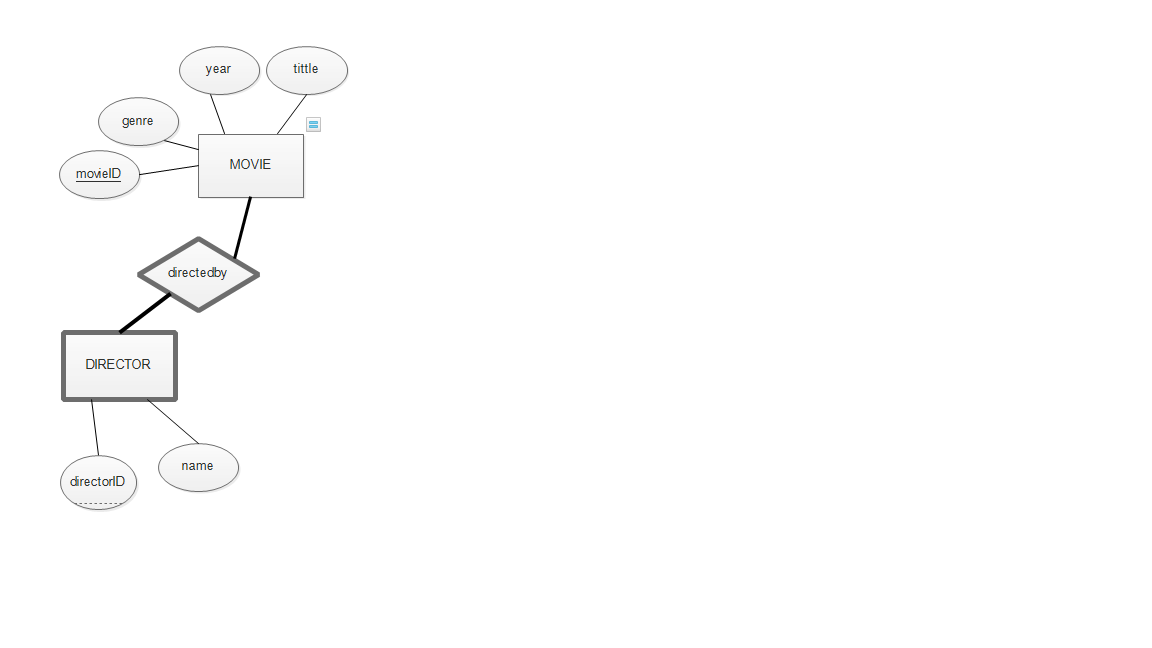
\includegraphics[scale=0.3]{movie-director.png}
Explanation related to user scenario: movie directed by director relation , weak entity.
when movie gets deleted we take everything that comes with that movie, director.
For the first moviegoer scenario, selecting a movie. The movie relation is used in the diagram, it has the attributes that a user would need. The movie table would have movieID, genre, year, and title and director has name and director ID
when selecting a movie you can also select by director 
\item{ }
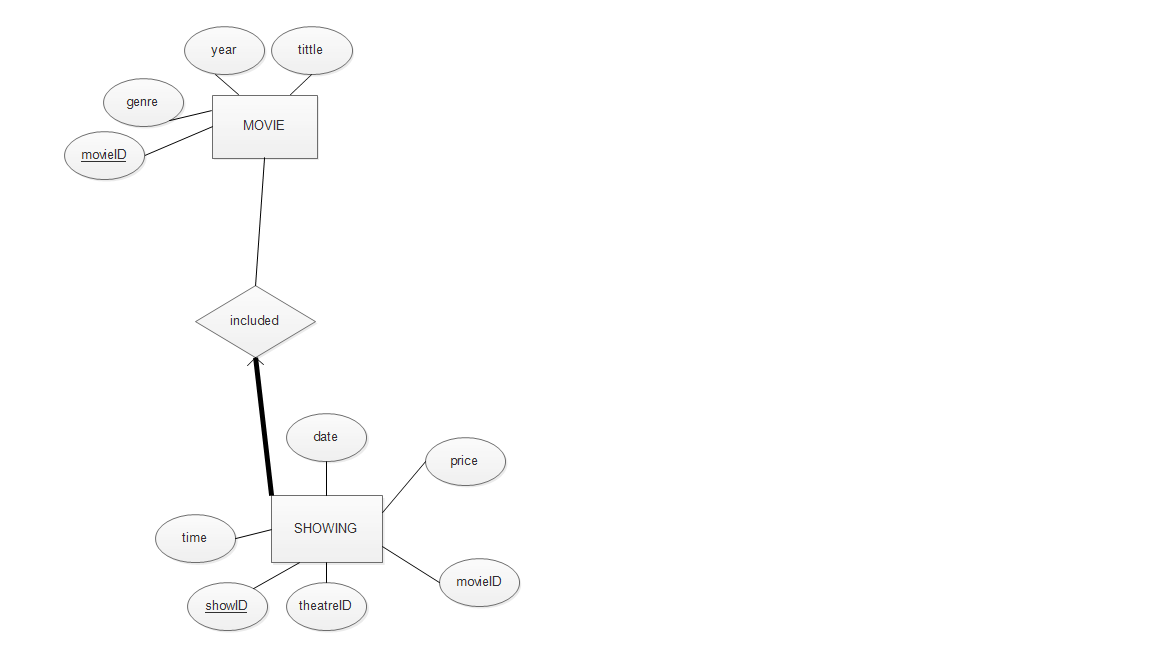
\includegraphics[scale=0.3]{MovieofShowing.png}
explanation related to user scenario: showing of one movie. For the ticket seller scenario, he/she is approached by a moviegoer who purchased the wrong ticket for the wrong showing. Showing has attributes that would enable this transaction. 
\item{ }
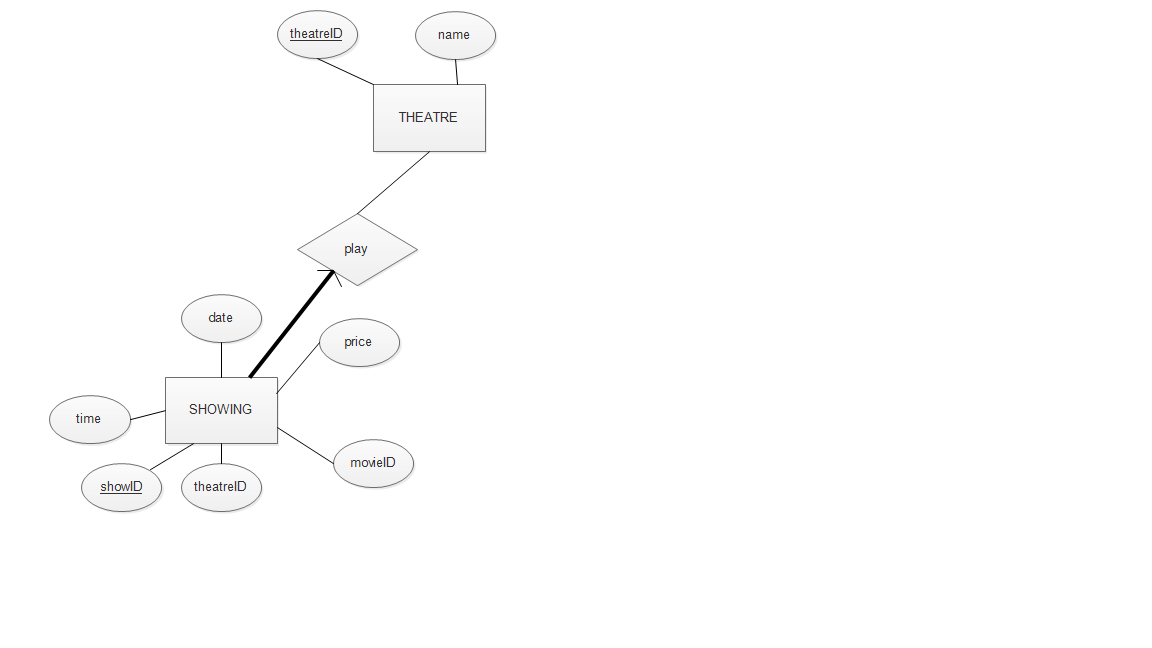
\includegraphics[scale=0.3]{ShowingPlayedinTheatre.png}
explanation related to user scenario: For the showing manager scenario , it states that the theater manager has the ability to remove a showtime of a movie. this relation shows theater attributes and showing attributes that can allow the showing manager to remove showtimes 
\item{ }
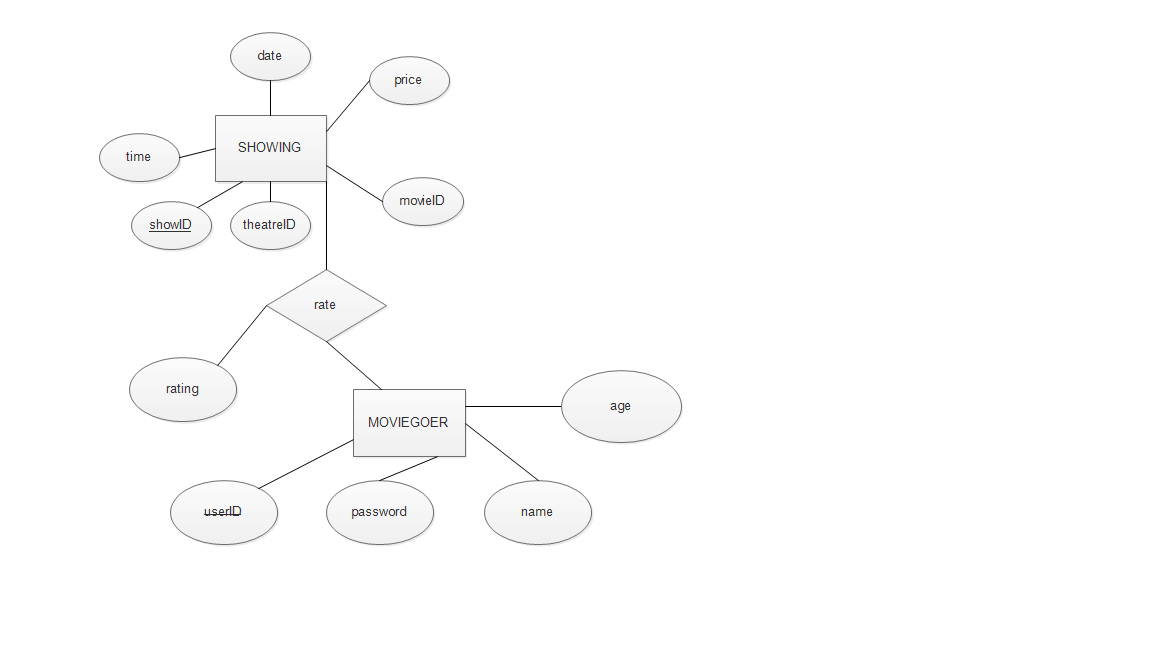
\includegraphics[scale=0.3]{MoviegoerrateShowing.png}
explanation related to user scenario: moviegoer can rate showing , each of their attributes allow a user to rate a showing by movie ID 
\item{ }
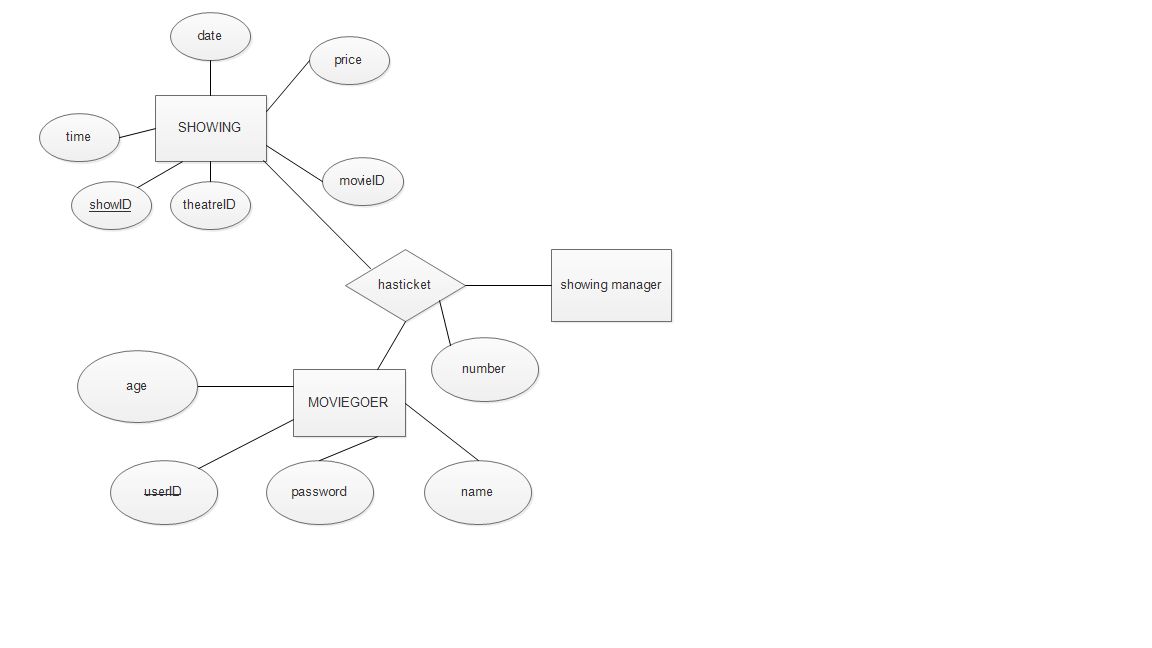
\includegraphics[scale=0.3]{MoviegoerhasticketShowing.png}
explanation related to user scenario: This ternary relationship is between ticket seller  , moviegoer and showing . For the ticket seller scenario, he/she is approached by a moviegoer who purchased the wrong ticket for the wrong showing.The ticket seller has access to the user accounts, and it is depicted in the relationship has ticket between showing and moviegoer because the tickets seller has all tickets of the moviegoer and is able to change it.
\item{ }
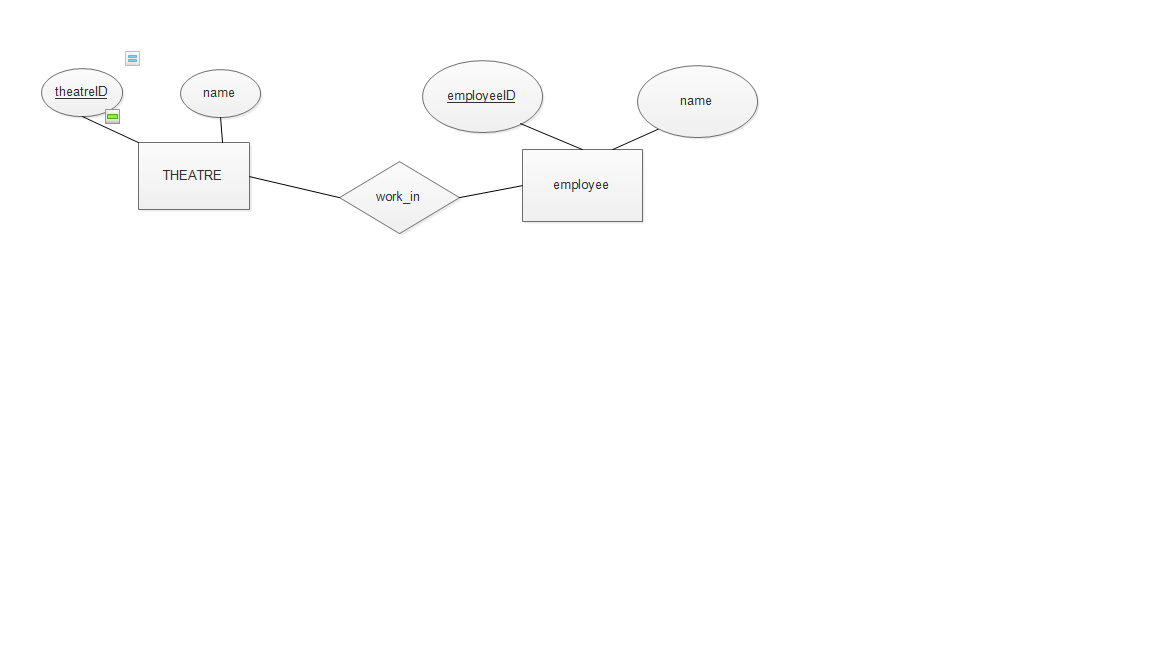
\includegraphics[scale=0.3]{TheatrehasEmployee.png}
explanation related to user scenario: many employees work in each theater ,relationship called employeeWorkin, the most important employees being ticket seller, chain manager, showing manager, and theater manager
\item{ }
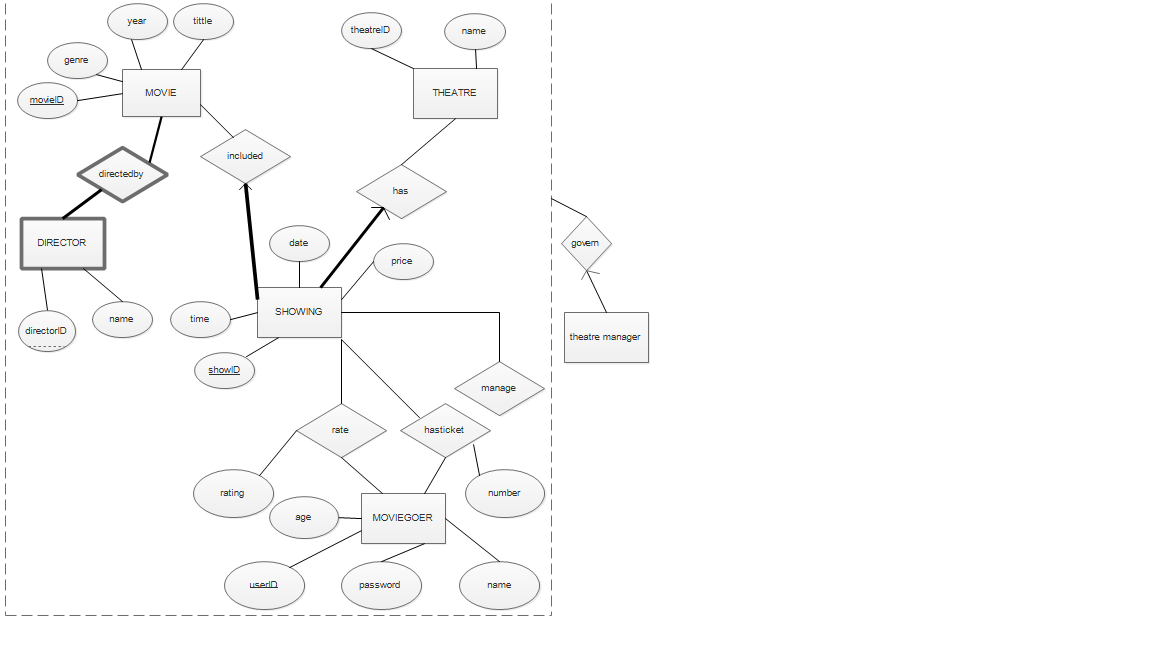
\includegraphics[scale=0.3]{theatremanagergovern.png}
explanation related to user scenario: a theatre manager of that theatre can manage all the stuff in that theatre, including showing, movie, and moviegoer.
\item{ }
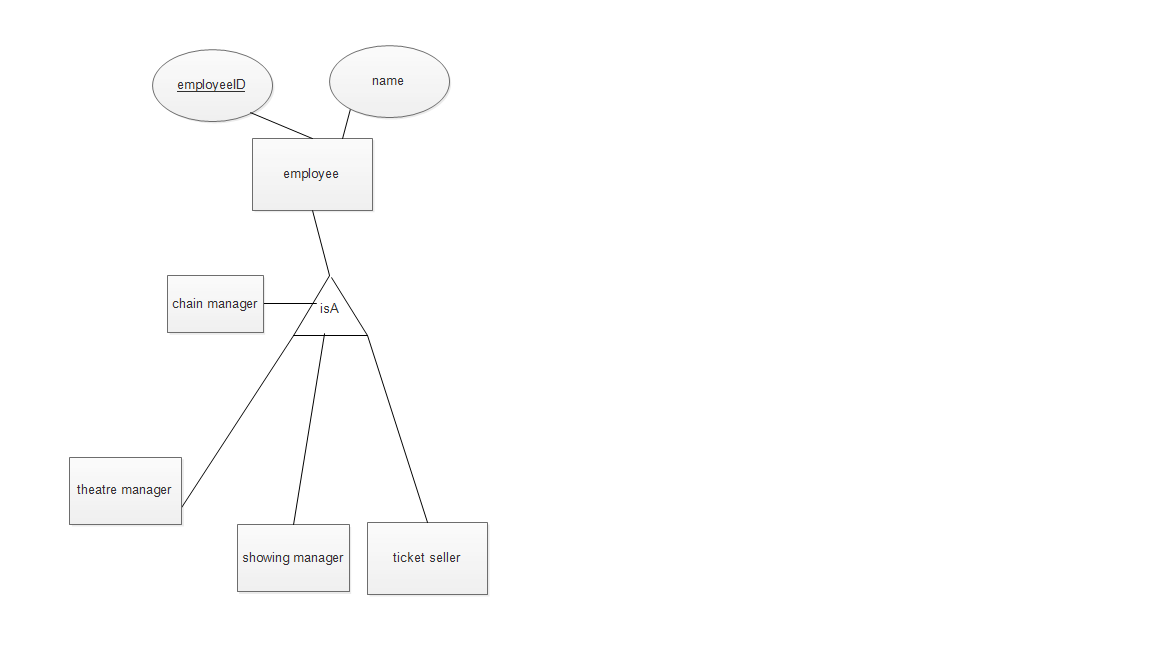
\includegraphics[scale=0.3]{isA.png}
explanation related to user scenario: ticket seller, chain manager, showing manager, and theater manager are different types of employee. Each of them has different authority
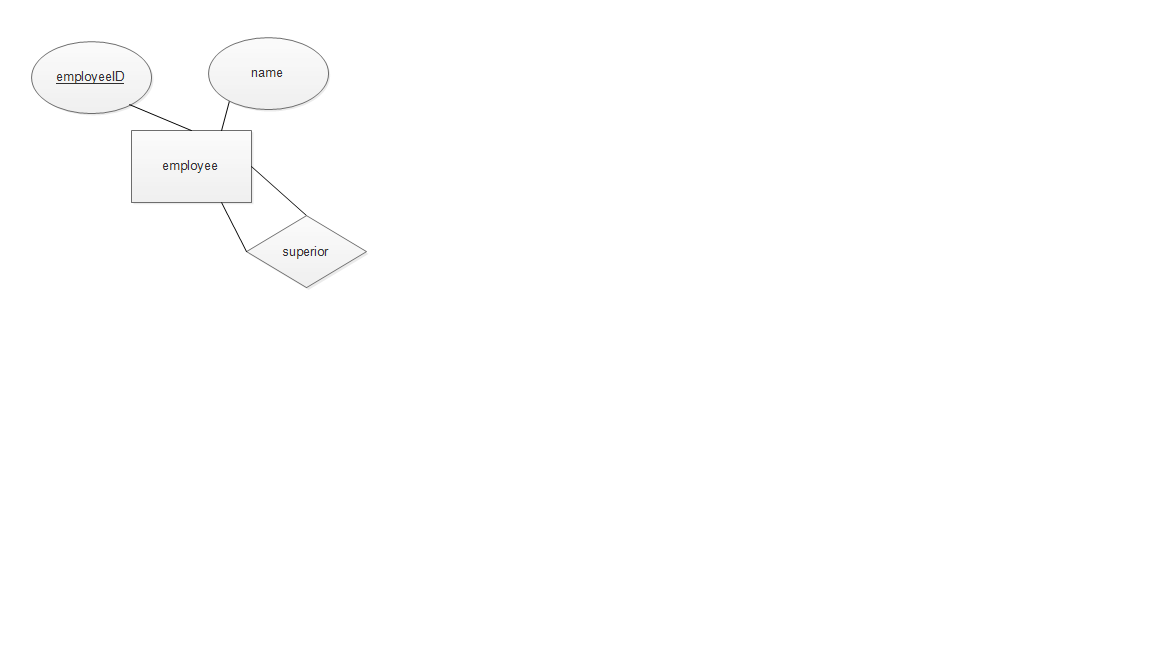
\includegraphics[scale=0.3]{superior.png}
explanation related to user scenario: each employee may be superior to other employees. It's a unary relationship.
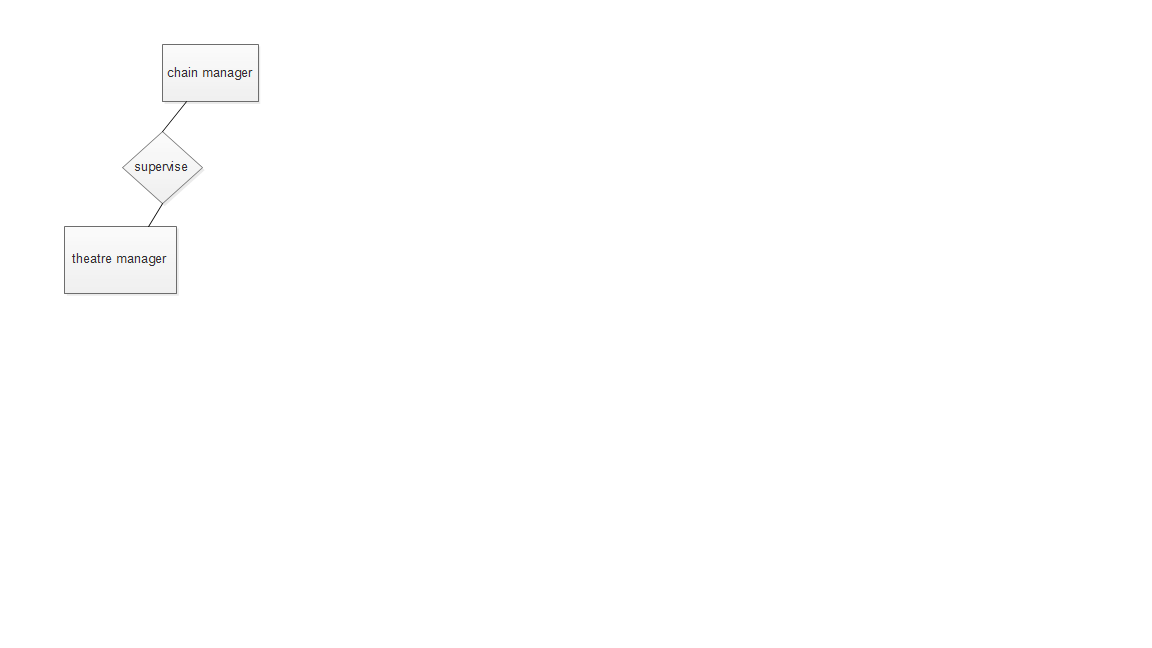
\includegraphics[scale=0.3]{supervise.png}
explanation related to user scenario: Chain manager supervise all the theatre manager in that chain.
\end{itemize}
\begin{itemize} 
\item{ The ER diagram in its entirety: }
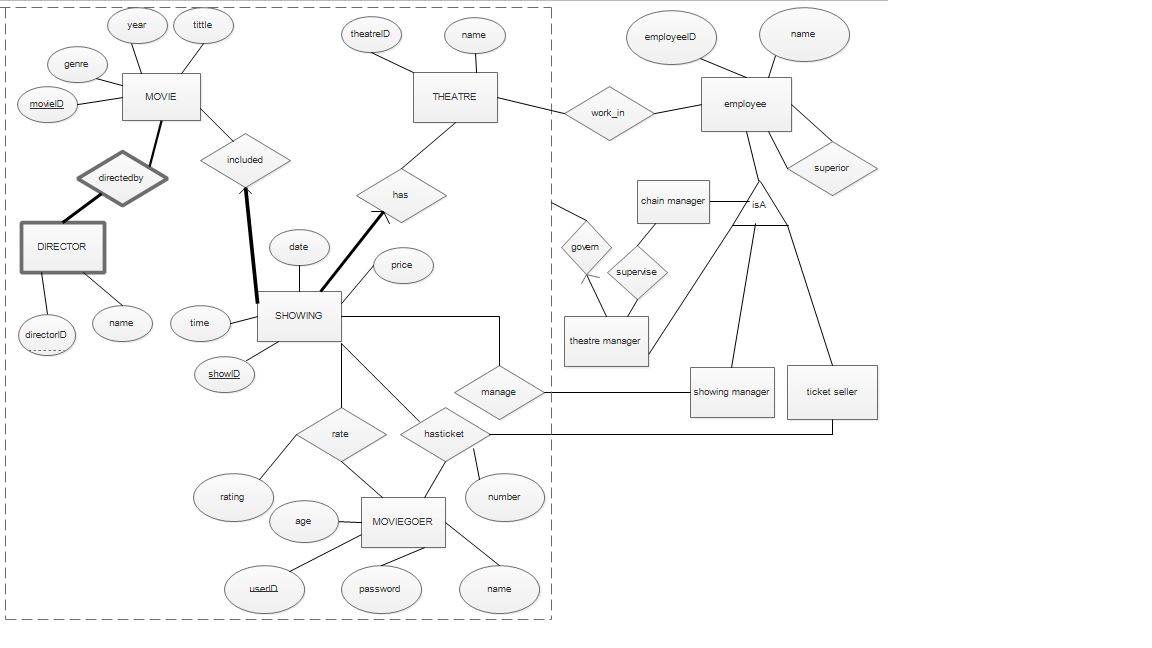
\includegraphics[scale=0.3]{ERmodel.png}
\item{ The ER diagram description (corresponding to the user scenarios): }
For the moviegoer scenario the moviegoer logs into his/her account and selects a movie and buys ticket(s). The relationship between showing and moviegoer depicts this relationship. The attributes in showing are needed to buy a ticket. The attributes for showing are time, showID, theaterID, movieID, price, and date and each attribute is used in this transaction.For selecting a movie the movie relation is used in the diagram, it has the attributes that a user would need. The movie table would have movieID, genre, year, and title.The relationship between moviegoer and showing displays that the moviegoer has a ticket for the chosen showing the moviegoer picked. The moviegoer's attributes are what we need to make this happen , which leads into the second user scenario.
For the moviegoer to register in our system we would need the userID, password, and name. To buy a ticket a user would have to register in the system therefore these attributes for moviegoer are important.
\item{ }
For the chain manager scenario , the chain manager adds employees to the database. The relationship between employee and theater depicts this scenario. The employee relation has an attribute ,employeeID. which is essential to this scenario because the theater has lots of employees working for them but every person working for the theaters are employees, that is why we use the is A relationship between them all , if not a theater manager , ticket seller, or administrator then its just a regular employee which is the other employees working at the theatre.
For the second scenario , it states that the showing manager has the ability to remove a showtime of a movie, the manage relationship between showing and theater manager, the attributes for the showing relation has time and date and it can be changed by the theater manager.
\item{ }
For the ticket seller scenario, he/she is approached by a moviegoer who purchased the wrong ticket for the wrong showing.The ticket seller has access to the user accounts, and it is depicted in the relationship has ticket between showing and moviegoer because the tickets seller has all tickets of the moviegoer and is able to change it.
For the second scenario, it states that the ticket seller wants to see if  a particular movie is doing well. The ticket seller is able to do this because he/she has access , by the has tickets relationship, to the showing table, where he/she can look up a movie and its ticket sales
\item{ }
For the theater manager scenario, the first scenario states that the theater manager taking out all showings of a certain movie. For this the theater manager has needs and has access to ticket sales, and showings. The theater manager is the administrator and has access to everything, relations such as movie, director, showing, theater,and moviegoer and employees because of the relationship between theater and employees. Theres an aggregation in the diagram to depict this administrator manage relationship.
The second scenario for the chain manager/administrator is he/she wants to see if a movie showing in one theater is worth showing in other branches. Again the administrator has access to information of all cinemas. in the showing relation the admin has access to rating because of the rate relationship between moviegoer and showing which has an attribute of rating. Therefore the administrator can find out the ratings of any showing as well as ticket sales because of the has ticket relationship and its number attribute which is between showing and moviegoer.
\item{ The integrity constraints defined in the ER diagram: }
Please insert the integrity constraints in here:
\begin{itemize} 
\item{ Integrity Constraint: }
Each showing must be of exactly one movie.
\item{ The description and justification of the integrity constraint: }
 A showing, by definition, is a specific movie being shown in a specific place at a specific time.  By this definition, there has to be a movie to be shown.  There cannot be more than one movie because an audience does not watch multiple movies at once.
\end{itemize}
\begin{itemize} 
\item{ Integrity Constraint: }
Each showing has exactly one theater.
\item{ The description and justification of the integrity constraint: }
 A showing, by definition, is a specific movie being shown in a specific place at a specific time.  The theater is that specific place, and so there can only be one.  And there has to be one, because there needs to be somewhere for the movie to be shown.
\end{itemize}
\begin{itemize} 
\item{ Integrity Constraint: }
Each movie has at least one director.
\item{ The description and justification of the integrity constraint: }
Every movie that exists was directed by someone.  However, it is possible for multiple people to co-direct.
\end{itemize}
\begin{itemize} 
\item{ Integrity Constraint: }
Each director has at least one movie.
\item{ The description and justification of the integrity constraint: }
 By definition, to be a director that person must have directed something.  Furthermore, there is no reason to store a director unless they belong to a movie the theater is storing information on.  It is possible for a director to have directed multiple movies.
\end{itemize}
\begin{itemize} 
\item{ Integrity Constraint: }
movieID is the primary key for a movie.
\item{ The description and justification of the integrity constraint: }
All entities need a key, and no movie trait is guaranteed to be unique (two movies can share a title, for example), so a unique ID number needs to be created for each movie.
\end{itemize}
\begin{itemize} 
\item{ Integrity Constraint: }
showId is the primary key for a showing.
\item{ The description and justification of the integrity constraint: }
All entities need a key, and no showing trait is guaranteed to be unique- one theater could have two showings of the same movie at the same time.  For this reason, a unique ID number needs to be created for each showing.
\end{itemize}
\begin{itemize} 
\item{ Integrity Constraint: }
userID is the primary key for a moviegoer.
\item{ The description and justification of the integrity constraint: }
All entities need a key, and no moviegoer trait is guaranteed to be uniquie (two moviegoers can have the same name, for example), so a unique ID number needs to be created for each moviegoer.
\end{itemize}
\begin{itemize} 
\item{ Integrity Constraint: }
theaterID is the primary key for a theater.
\item{ The description and justification of the integrity constraint: }
All entities need a key.  Since there is no other information stored for a theater that is uniquely identifying, so an ID number must be created for that purpose.
\end{itemize}
\begin{itemize} 
\item{ Integrity Constraint: }
employeeID is the primary key for an employee.
\item{ The description and justification of the integrity constraint: }
Just like with moviegoers, it is possible for multiple employees to share a name or other attributes, so a unique ID number is necessary for each employee
\end{itemize}
\begin{itemize} 
\item{ Integrity Constraint: }
Each theater manager can manage at most one theater.
\item{ The description and justification of the integrity constraint: }
 A manager of multiple theaters is a different job (admin).  A manager typically manages exactly one theater, but it is possible for a manager to not yet be assigned a theater, or to be a substitute and not belong to a specific theater.
\end{itemize}
\end{itemize}
}


\subsection{Stage3 - The Implementation Stage. }\label{sec: 3 The Implementation Stage.}
%%%%%%%%%%%%%%%%%%%%%%%%%%%%%%%%%%%%%%%%%%%%%%%%%%%%%%%%%%%%%%%%%%%%%%%%%%%%%%%%%%%%%%%%%%%%%%%%%%%%%%%%%%
\textnormal{
Building the corresponding relational tables, according to the proposed ER model described in the previous phase enforcing the different integrity constraints.  
The deliverables for this stage include the following items (Please refer to the original Project Description for more details):
\begin{itemize} 
\item{}
The SQL tables that represent the ER project model, along with at least 3-5 rows of concrete data per table.
\item{}
The normalization steps for each table, along with explanations/justifications of each normalization step.
\item{}
The SQL table after the normalization steps (showing all table attributes).
\item{}
The SQL statements used to create the SQL tables, including the required triggers as well as the integrity constraints. At least 2 triggers and 2 of each of the following constraint types have to exist in the project tables overall: 
\begin{itemize} 
\item{}
	Data-range constraints for certain fields (for example: the age field should be between 10 and 99, while all other entries should be rejected by the system).
\item{}
	Whether some users will be denied access and/or updates to some data according to their roles (for example: student1 can not access other students' ' grades, so a violation error pops up upon that action. Another example: a sales person can see an item price, but can not change it, since only a manger can, also a violation error pops up upon that update attempt).
\end{itemize}
\item{}
So each table should be followed by the following items:
\begin{itemize} 
\item{}
	Explanation for each constraint, providing examples of certain data access and/or update restrictions per user type. 
\item{}
	Explanation/justification for each trigger, providing examples of certain data access and/or updates per user type. 
\end{itemize}
\end{itemize}
Please insert your deliverables for Stage3 as follows:
\begin{itemize} 
\item{ The SQL Table, including data entries: }
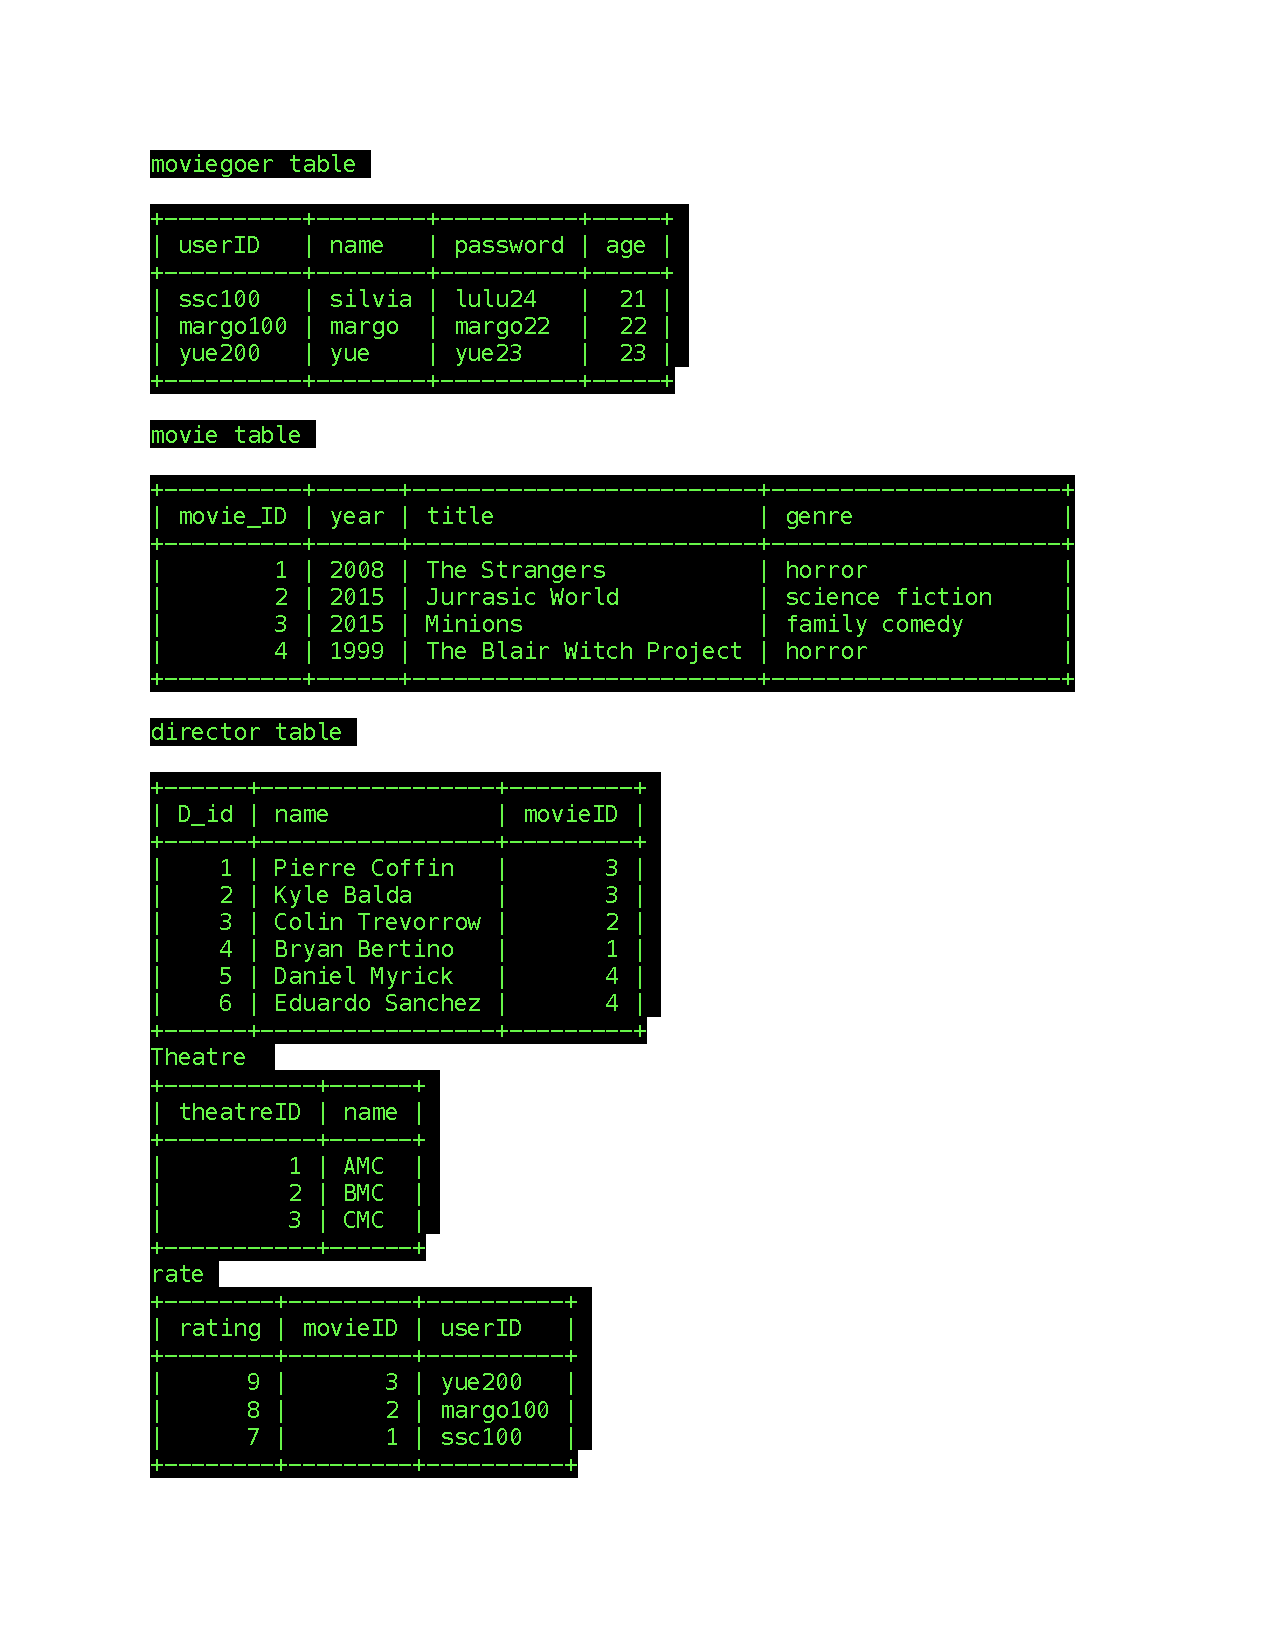
\includepdf[pages={1,2,3}]{tables.pdf}
\item{The normalization steps for each table, along with explanations/justifications: }
The normalization steps should be inserted as follows.
\begin{itemize} 
	\item{The normalization step for the SQL table: }
	Theater Normalization already in 3NF
	\item{The explanations/justification of the normalization step: }
	 It passes 1NF because each attribute can only have one value in a given row. Each theater has one ID and one name.  It passes 2NF and 3NF because the only non-key attribute, name, attribute follows from the theaterID, which is the primary key.
\end{itemize}
\begin{itemize} 
	\item{The normalization step for the SQL table: }
	Showing Normalization already in 3NF
	\item{The explanations/justification of the normalization step: }
	 It passes 1NF because each attribute can only have one value in a given row. Each showing has only one ID, place, date, time, and movie being shown.  It passes 2NF and 3NF because the non-key attributes depend on the entire primary key alone.  The place, date, time, and movie are all independent from each other, and only follow from the showID.
\end{itemize}
\begin{itemize} 
	\item{The normalization step for the SQL table: }
	HasTicket Normalization already in  3NF
	\item{The explanations/justification of the normalization step: }
	 It passes 1NF because each attribute can only have one value in a given row.  Each row consists of only one moviegoer with one amount of tickets for one showing.  It passes 2NF and 3NF because the non-key attribute, number of tickets, depends on the entire primary key alone.  The number of tickets relies on being for a particular moviegoer to use at a particular showing- in other words, both parts of the primary key.
\end{itemize}
\begin{itemize} 
	\item{The normalization step for the SQL table: }
	Rate Normalization already in 3NF
	\item{The explanations/justification of the normalization step: }
	It passes 1NF because each attribute can only have one value in a given row. Each rate consists of 		one rating from one moviegoer for one movie. It passes 2NF and 3NF because the non-key attribute, 	rating, depend on the entire primary key alone.   The rating is from a specific moviegoer for a specific 	movie, so it relies on both parts of the primary key.
\end{itemize}
\begin{itemize} 
	\item{The normalization step for the SQL table: }
	moviegoer Normalization already in 3NF
	\item{The explanations/justification of the normalization step: }
	it passes 1NF because each attribute can only have one value in each row. Each moviegoer has a 		unique userID. it passes 2NF and 3NF because the non key attributes depend on the entire primary 		key alone. super key being movie ID . year, title and genre are all independent from each other 
\end{itemize}
\begin{itemize} 
	\item{The normalization step for the SQL table: }
	movie Normalization already in 3NF
	\item{The explanations/justification of the normalization step: }
	it passes 1NF because each attribute can only have one value in each row. Each movie has a 		unique movie ID. . it passes 2NF and 3NF because the non key attributes depend on the entire primary 		key alone. primary key being user ID . name, password, and age are all independent from each other 
\end{itemize}
\begin{itemize} 
	\item{The normalization step for the SQL table: }
	director Normalization already in 3NF
	\item{The explanations/justification of the normalization step: }
	it passes 1NF because each attribute can only have one value in each row. Each director has a unique director ID.  It passes 2NF and 3NF because the non-key attribute, rating, depend on the entire primary key alone. There can be many directors for a movie so the director is from a specific movie and has a unique Director ID 
\end{itemize}
\begin{itemize} 
	\item{The normalization step for the SQL table: }
	Employee Normalization already in 3NF
	\item{The explanations/justification of the normalization step: }
	It passes 1NF because each attribute can only have one value in a given row. Each employee has one ID one type and one name.� It passes 2NF and 3NF because the non-key attributes, name and type, attribute follows from the EmployeeID, which is the primary key
\end{itemize}
\begin{itemize} 
	\item{The normalization step for the SQL table: }
	employeeWorkin Normalization already in 3NF
	\item{The explanations/justification of the normalization step: }
	It passes 1NF because each attribute can only have one value in a given row. Each hasEmployee has only one theatreID and employeeID being shown.� It passes 2NF and 3NF because there is no non-key attributes in the table. 
\end{itemize}
\begin{itemize} 
	\item{The normalization step for the SQL table: }
	Theatremanagedby Normalization already in 3NF
	\item{The explanations/justification of the normalization step: }
	It passes 1NF because each attribute can only have one value in a given row. Each Theatremanagedby has only one theatreID and theatremanagerID being shown.� It passes 2NF and 3NF because there is no non-key attributes in the table. 
\end{itemize}
\begin{itemize} 
	\item{The normalization step for the SQL table: }
	govern Normalization already in 3NF
	\item{The explanations/justification of the normalization step: }
	It passes 1NF because each attribute can only have one value in a given row.  It passes 2NF and 3NF because there is no non-key attributes in the table. the attributes are all foreign keys 
\end{itemize}
\begin{itemize} 
	\item{The normalization step for the SQL table: }
	supervise Normalization already in 3NF
	\item{The explanations/justification of the normalization step: }
	It passes 1NF because each attribute can only have one value in a given row. It passes 2NF and 3NF because there is no non-key attributes in the table. 
\end{itemize}
\begin{itemize} 
	\item{The normalization step for the SQL table: }
	Showingmanagedby Normalization already in 3NF
	\item{The explanations/justification of the normalization step: }
	 It passes 1NF because each attribute can only have one value in a given row. Each Showingmanagedby has only one showingID and showingmanagerID being shown.� It passes 2NF and 3NF because there is no non-key attributes in the table
\end{itemize}
\begin{itemize} 
	\item{The normalization step for the SQL table: }
	superior Normalization already in 3NF
	\item{The explanations/justification of the normalization step: }
	  It passes 1NF because each attribute can only have one value in a given row. Each superior has only one employeeID and supervisorID being shown.� It passes 2NF and 3NF because the non-key attributes, supervisorID, attribute follows from the employeeID, which is the primary key
\end{itemize}
\item{The SQL statement to create the table: }
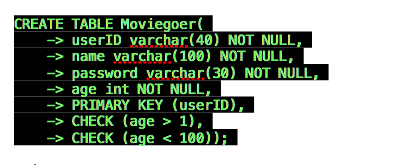
\includegraphics[scale=0.3]{moviegoertable.png}
\item{The Triggers used in the statement: }
Please insert the triggers are as follows:
\begin{itemize} 
	\item{The Trigger: }
	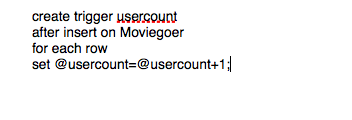
\includegraphics[scale=0.3]{usercount.png}
	\item{The Trigger Explanation/Justification: }
	a count that is added 1 after every insert on the moviegoer table to count how many moviegoers are in the system
	\item{The Trigger Examples (in correlation with the user(s) interaction with the system): }
	the theater manager wants to see how many moviegoers are in his theater ,he can just summon this trigger customer count
\end{itemize}
\item{The Data Range Constraints used in the statement: }
Please insert the Data Range Constraints as follows:
\begin{itemize} 
	\item{The Data Range Constraint: }
	Age in the moviegoer table must be between 1 and 100
	\item{The Data Range Constraint Explanation:}
	ages 1 to 100 are common for a typical person
	\item{The Data Range Constraint Example(s) (in correlation with the user(s) interaction with the system): } 
	A person who is 25, puts their age as 25 and is accepted and valid another example is if the user puts in 255 but the last 5  is put in by mistake, the system will not take age 255 so the insert is invalid
	\item{The Data Access/update Constraint: }
	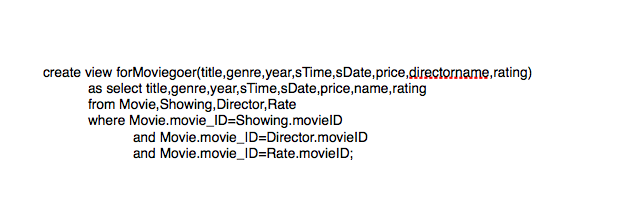
\includegraphics[scale=0.3]{moviegoerview.png}
	\item{The Data Access/update Constraint Explanation:}
	For the moviegoer view , the moviegoer (client) cannot look at other users ID or passwords, name of employees or what type is each employee therefore, we create a view solely for the moviegoer , so they can have access to the movie titles, year, genre, date, time,directors, price and theater name so the moviegoer is able to search movies by director, by title, by date, time and a moviegoer is also able to see price so they can buy tickets 
	\item{The Data Access/update Constraint Example(s) (in correlation with the user(s) interaction with the system): } 
	When a moviegoer goes to buy a ticket  and wants to search by title.They search by title ?the strangers ? and find the times for it and price and go ahead and buy the ticket 
	\item{The Data Access/update Constraint: }
	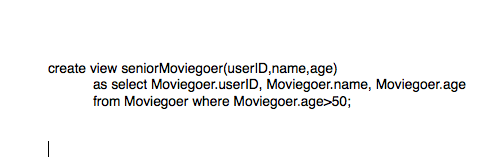
\includegraphics[scale=0.3]{seniormoviegoer.png}
	\item{The Data Access/update Constraint Explanation:}
	The senior moviegoer view is for employees , so they know who is a senior out of their customers , so they can get benefits , such as lower ticket price.
	\item{The Data Access/update Constraint Example(s) (in correlation with the user(s) interaction with the system): } 
	For example if its senior Day , which is when seniors get a free movie ticket to any movie , the theater can give it to them based on this view. This view lists all senior users that exist.  
\end{itemize}
\item{The SQL statement to create the table: }
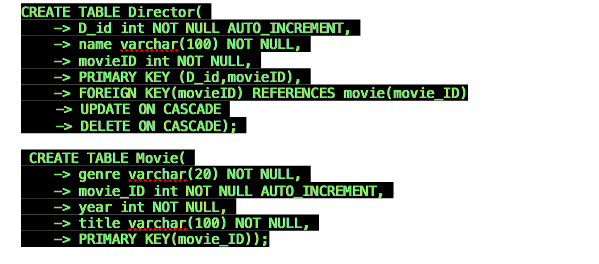
\includegraphics[scale=0.3]{tables1.png}
\item{The Triggers used in the statement: }
Please insert the triggers are as follows:
\begin{itemize} 
	\item{The Trigger: }
	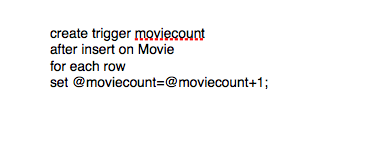
\includegraphics[scale=0.3]{moviecount.png}
	\item{The Trigger Explanation/Justification: }
	a count variable in which one is added every time a movie is added to the system so any of the managers can know how many movies are added to their movie theater system.
	\item{The Trigger Examples (in correlation with the user(s) interaction with the system): }
	a theater manager wants to know how many movies his theater has
\end{itemize}
\item{The SQL statement to create the table: }
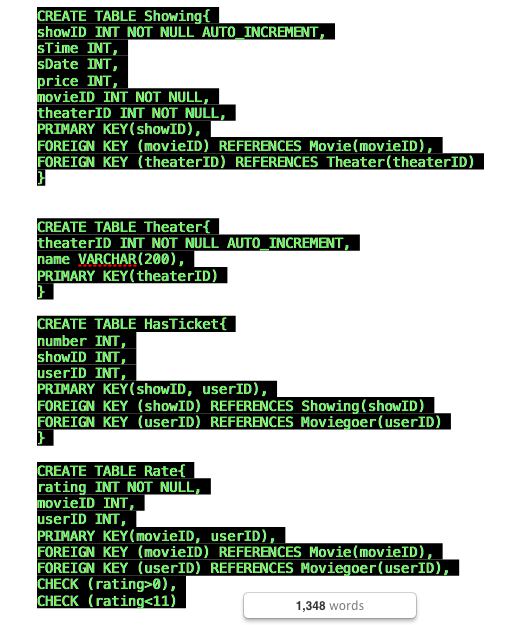
\includegraphics[scale=0.3]{tables2.png}
\item{The Data Range Constraints used in the statement: }
Please insert the Data Range Constraints as follows:
\begin{itemize} 
	\item{The Data Range Constraint: }
	A rating in the 'rate' table must be between one and ten.  
	\item{The Data Range Constraint Explanation:}
	 A ten point scale is a common one for movie ratings, with 10 being the highest possible rating (the movie was fantastic) and one being the lowest (the movie was terrible).  A movie must be rated within the scale for the information to be useful.
	\item{The Data Range Constraint Example(s) (in correlation with the user(s) interaction with the system): } 
	A moviegoer tries to rate a movie they love a 15, but it is rejected because it is off the rating scale.  They then rate the movie 10, and it is accepted.
\end{itemize}
\item{The SQL statement to create the table: }
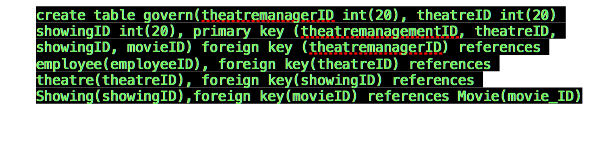
\includegraphics[scale=0.3]{create.png}
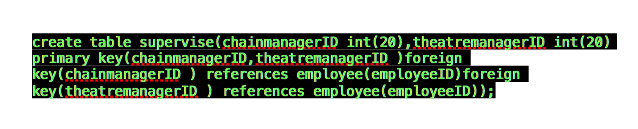
\includegraphics[scale=0.3]{create1.png}
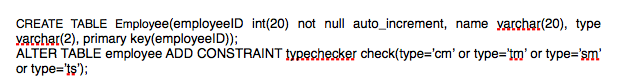
\includegraphics[scale=0.3]{emptables.png}
\item{The Data Range Constraints used in the statement: }
Please insert the Data Range Constraints as follows:
\begin{itemize} 
	\item{The Data Range Constraint: }
	 type must be one of the following cm, tm, sm or ts. 
	\item{The Data Range Constraint Explanation:}
	 an employee can only be a chain manager or ticket seller or theater manager or showing manager
	\item{The Data Range Constraint Example(s) (in correlation with the user(s) interaction with the system): } 
	 the chain manager puts tp for a sm (showing manager )by mistake , the insert is not allowed because tp doesn't exist
\end{itemize}
\item{The SQL statement to create the table: }
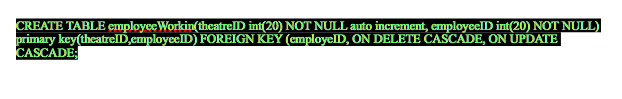
\includegraphics[scale=0.3]{sqlstatementempw.png}
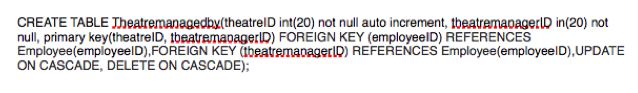
\includegraphics[scale=0.3]{theaterM.png}
\item{The Data Range Constraints used in the statement: }
Please insert the Data Range Constraints as follows:
\begin{itemize} 
	\item{The Data Access/update Constraint: }
	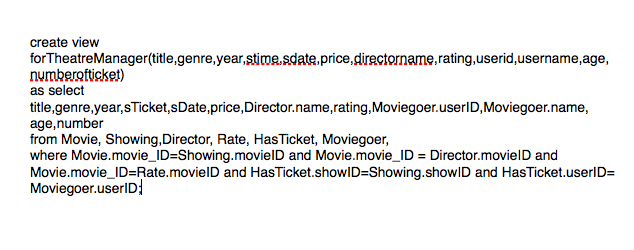
\includegraphics[scale=0.3]{forTheaterManager.png}
	\item{The Data Access/update Constraint Explanation:}
	For the theater manager view , the theater manager has access to everything in the database except the employees , because the chain manager takes care of that .The theatre manager can look up  cannot look at other users ID or passwords, name of employees or what type is each employee 
therefore, we create a view solely for the theater manager , so they can have access to the movie, showings, moviegoer entities so the theater manager can make any changes they want to movies in the system, showings and can make changes to the users in the system
	\item{The Data Access/update Constraint Example(s) (in correlation with the user(s) interaction with the system): } 
	When a theater manager wants to erase a showtime of a movie , it has access to do that , and other people cant
\end{itemize}
\item{The SQL statement to create the table: }
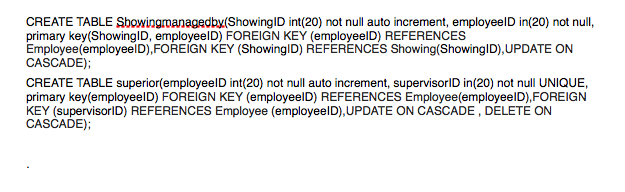
\includegraphics[scale=0.3]{last2tables.png}
\end{itemize}
Repeat that pattern for every table created.
}


\subsection{Stage4 -	User Interface. }\label{sec: 4.	User Interface.}
%%%%%%%%%%%%%%%%%%%%%%%%%%%%%%%%%%%%%%%%%%%%%%%%%%%%%%%%%%%%%%%%%%%%%%%%%%%%%%%%%%%%%%%%%%%%%%%%%%%%%%%%%%
\textnormal{
Describing of a User Interface (UI) to the system along with the related information that will be shown on each screen (How users will query the tables and view the query results). The emphasis should be placed on the process required for a user in order to meet a particular information need, in a user-friendly manner.
The deliverables for this stage include the following items (Please refer to the original Project Description for more details):
\begin{itemize} 
\item{}
	The SQL statements used to query the data. 
\item{}
	The error messages that will pop-up when users access and/or updates are denied.
\item{}
	The error messages corresponding to the integrity constraints violations.
\item{}
	The error messages corresponding to the data range constraints violations.
\item{}
	The header of the views created in order to facilitate data accesses, according to users'  needs. 
\item{}
	Each view created must be justified. Any triggers built upon those views should be explained and justified as well. At least one view should be created and justified for the project.
\end{itemize}
Please insert your deliverables for Stage4 as follows:
\begin{itemize} 
\item{The the first SQL statement used to query the data: }
	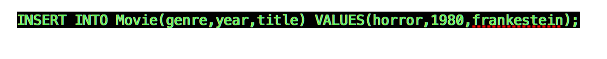
\includegraphics[scale=0.3]{insert1.png}
\item{The tables taking part in the query statement (table names and headers): }
	Please insert the tables taking part in the query statement, as follows.
	 \begin{itemize} 
	 \item{The name of the first table taking part in the query: }
	 Movie
	  \item{The header of the table  (all attributes): }
	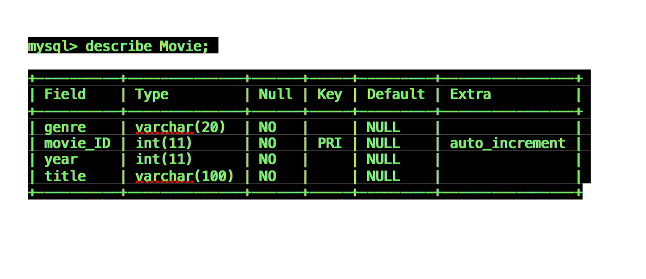
\includegraphics[scale=0.3]{describemovie.png}
	  \item{The attributes of the table taking part in the query: }
	  genre,year,title
	 \end{itemize}
\item{}
	The error messages popping-up when users access and/or updates are denied (along with explanations and examples):
	\begin{itemize} 
	\item{The error message: }
	ERROR 1142(42000): INSERT command denied to user ?moviegoer?@?localhost? for table ?Movie?
	\item{The error message explanation (upon which violation does it take place): }
	When a moviegoer tries to make changes to the movie information, this will be denied because the moviegoer does not have access to movie information
	\item{The error message example according to user(s) scenario(s): }
	When a moviegoer user tries to make add a movie to the movie table because he wants to add one of his favorite movies that arent showing in any of theaters , he/she tries to add it and the error message will pop-up.
	 \end{itemize}
\item{The the first SQL statement used to query the data: }
	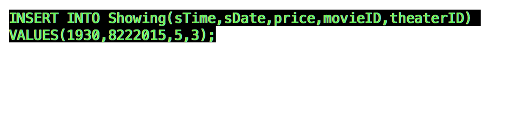
\includegraphics[scale=0.3]{insert2.png}
\item{The tables taking part in the query statement (table names and headers): }
	Please insert the tables taking part in the query statement, as follows.
	 \begin{itemize} 
	 \item{The name of the first table taking part in the query: }
	 Showing
	  \item{The header of the table  (all attributes): }
	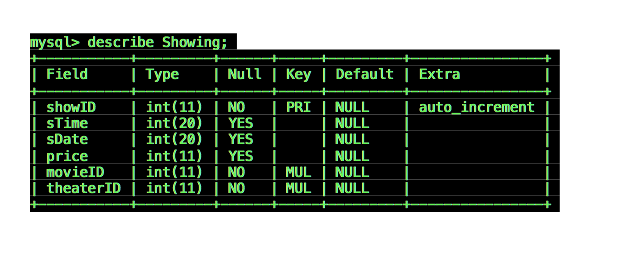
\includegraphics[scale=0.3]{desshowing.png}
	  \item{The attributes of the table taking part in the query: }
	  showID,sTime,sDate,price,movieID,theaterID
	 \end{itemize}
\item{}
	The error messages popping-up when users access and/or updates are denied (along with explanations and examples):
	\begin{itemize} 
	\item{The error message: }
	 ERROR 1142(42000): INSERT command denied to user ?moviegoer?@?localhost? for table ?Showing?
	\item{The error message explanation (upon which violation does it take place): }
	When a moviegoer tries to make changes to the showing information, the require will be denied because the moviegoer do not have access to showing information
	\item{The error message example according to user(s) scenario(s): }
	When a moviegoer user tries to make changes to showing information to mess with one of the theaters, the error message will pop-up.
	 \end{itemize}
\item{The the first SQL statement used to query the data: }
	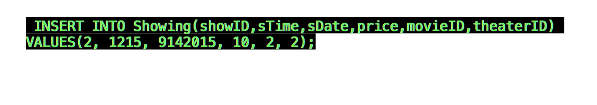
\includegraphics[scale=0.3]{IC.png}
\item{The tables taking part in the query statement (table names and headers): }
	Please insert the tables taking part in the query statement, as follows.
	 \begin{itemize} 
	 \item{The name of the first table taking part in the query: }
	Showing
	\item{The header of the table  (all attributes): }
	Showing(showID,sTime,sDate,price,movieID,theaterID)
	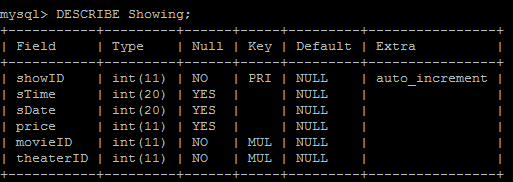
\includegraphics[scale=0.3]{m.png}
	  \item{The attributes of the table taking part in the query: }
	 showID,sTime,sDate,price,movieID,theaterID
	 \end{itemize}
	 Please repeat that pattern for all tables taking part in that query.
\item{}
	The error messages corresponding to the integrity constraints violations (along with explanations and examples).
	\begin{itemize} 
	\item{The error message: }
	"Cannot duplicate an ID; must be unique."
	\item{The error message explanation (upon which violation does it take place): }
	This error is for when a user tries to make a new movie showing with a showing ID that is already used for another showing.  This violates the primary key intergrity constraint.
	\item{The error message example according to user(s) scenario(s): }
	An employee tries to create a showing with an already existing ID.  The error message catches this and explains that each showing must have its own ID.
	 \end{itemize}
\item{The the first SQL statement used to query the data: }
	
\includegraphics[scale=0.3]{sql.png}
\item{The tables taking part in the query statement (table names and headers): }
	Please insert the tables taking part in the query statement, as follows.
	 \begin{itemize} 
	 \item{The name of the first table taking part in the query: }
	 Rate
	 \item{The header of the table  (all attributes): }
	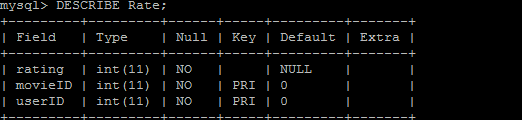
\includegraphics[scale=0.3]{mm.png}
	 \item{The attributes of the table taking part in the query: }
	  rating,movieID,userID
	 \end{itemize}
\item{}
	The error messages corresponding to the integrity constraints violations (along with explanations and examples).
	\begin{itemize} 
	\item{The error message: }
	Null was entered into a field that cannot be null
	\item{The error message explanation (upon which violation does it take place): }
	This error is for when a user tries to rate a movie without specifying a movie ID.  This violates the integrity constraint that each rating must be for exactly one movie.
	\item{The error message example according to user(s) scenario(s): }
	 A user enters a rating, but does not specify the movie that the rating is for.  Since the rating has to belong to a movie, that action is not allowed
	 \end{itemize}
\item{The the first SQL statement used to query the data: }
	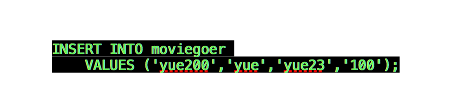
\includegraphics[scale=0.3]{insertData.png}
\item{The tables taking part in the query statement (table names and headers): }
	Please insert the tables taking part in the query statement, as follows.
	 \begin{itemize} 
	 \item{The name of the first table taking part in the query: }
	 Moviegoer
	  \item{The header of the table  (all attributes): }
	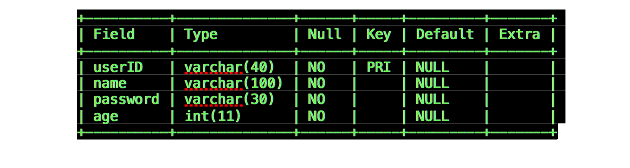
\includegraphics[scale=0.3]{moviegoerdescribe.png}
	  \item{The attributes of the table taking part in the query: }
	  userID, name, password, age
	 \end{itemize}
\item{}
	The error messages corresponding to the data range constraints violations (along with explanation).
	\begin{itemize} 
	\item{The error message: }
	invalid age
	\item{The error message explanation (upon which violation does it take place): }
	1 to 100 is accepted because a person who normally goes to movies can be between 1 and 100
	\item{The error message example according to user(s) scenario(s): }
	When a user types in their age when they are filling out their information we need, and they accidentally type 555 instead of 55 , the error message will pop up.
	 \end{itemize}
\item{The the first SQL statement used to query the data: }
	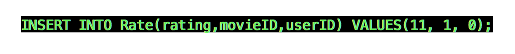
\includegraphics[scale=0.3]{ICC.png}
\item{The tables taking part in the query statement (table names and headers): }
	Please insert the tables taking part in the query statement, as follows.
	 \begin{itemize} 
	 \item{The name of the first table taking part in the query: }
	 Rate
	  \item{The header of the table  (all attributes): }
	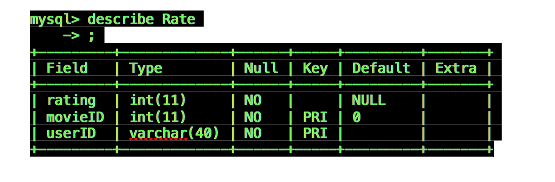
\includegraphics[scale=0.3]{rate.png}
	  \item{The attributes of the table taking part in the query: }
	  rating,movieID,userID
	  \end{itemize}
\item{}
	The error messages corresponding to the data range constraints violations (along with explanation).
	\begin{itemize} 
	\item{The error message: }
	invalid rating
	\item{The error message explanation (upon which violation does it take place): }
	rating is allowed from number 1 to 10 . if the moviegoer liked the movie then he/she would give it a 10 , otherwise if he/she did not like it at all they can give it a 1. rating between 1 and 10 no more or less, because it is usually one of the common scales out there, whereas if its 1 to 100 rating 
	\item{The error message example according to user(s) scenario(s): }
	if someone really liked a movie and wants to give them 100 rating , it will not be allowed because it would not be fair to the other movies, and it is not allowed because it is not the 1-10 common scale we are using for this theater management  
	 \end{itemize}
\item{The header of the views created in order to facilitate data accesses:}
Please insert the header of the views as follows:
\begin{itemize} 
	\item{The view created: }
	forMoviegoer
	\item{The view justification: }
	This view is built for moviegoer. When moviegoers log in, they have access to read all the movie information.
	\item{The tables taking part in the view and the specific attributes taking part in the view: }
	Please insert the tables names, headers, and the attributes as follows.
	\begin{itemize} 
		\item{The table name: }
		Movie
		\item{The table header (all attributes): }
		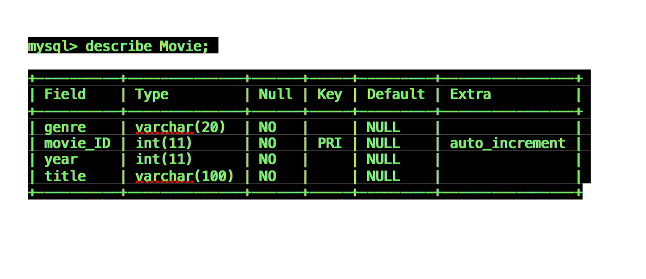
\includegraphics[scale=0.3]{describemovie.png}
		\item{The table attributes that take part in the view: }
		title, genre, year
	\end{itemize}
	\begin{itemize} 
		\item{The table name: }
		Showing
		\item{The table header (all attributes): }
		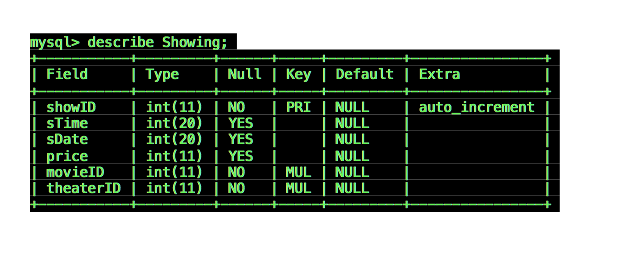
\includegraphics[scale=0.3]{desshowing.png}
		\item{The table attributes that take part in the view: }
		 sTime, sDate, price
	\end{itemize}
	\begin{itemize} 
		\item{The table name: }
		Director
		\item{The table header (all attributes): }
		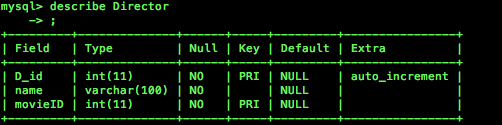
\includegraphics[scale=0.3]{director.png}
		\item{The table attributes that take part in the view: }
		directorname.
	\end{itemize}
	\begin{itemize} 
		\item{The table name: }
		Rate
		\item{The table header (all attributes): }
		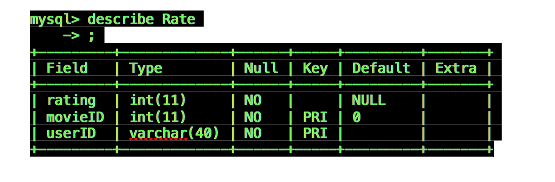
\includegraphics[scale=0.3]{rate.png}
		\item{The table attributes that take part in the view: }
		rating
	\end{itemize}
	Please repeat that pattern for every table that takes part in the view.
	\item{The SQL statement used for creating the view: }
	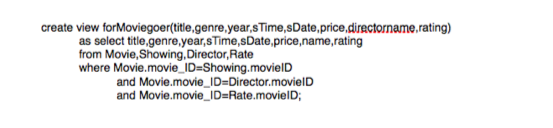
\includegraphics[scale=0.3]{VIEWMOVIEGOER.png}
	\item{The trigger built upon those views (if any): }
	Please insert the triggers as follows.
	\begin{itemize} 
		 \item{The trigger: }
		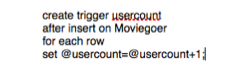
\includegraphics[scale=0.3]{trigger2.png}
		 \item{The trigger justification (explanation, correlating it to user scenario(s)): }
		a count that is added 1 after every insert on the moviegoer table to count how many moviegoers are in the system.the theater manager can see how many moviegoers are in his theater ?,he can just summon this trigger customer count 
 	\end{itemize}
\end{itemize}
Please, in case you have more than one view, repeat that pattern for each view.
\begin{itemize} 
	\item{The view created: }
	forTheatreManager
	\item{The view justification: }
	This view is built for theatre manager. When theatre manager log in, they have access to read all the movie information, showing information and the associated moviegoer information.
	\item{The tables taking part in the view and the specific attributes taking part in the view: }
	Please insert the tables names, headers, and the attributes as follows.
	\begin{itemize} 
		\item{The table name: }
		Movie
		\item{The table header (all attributes): }
		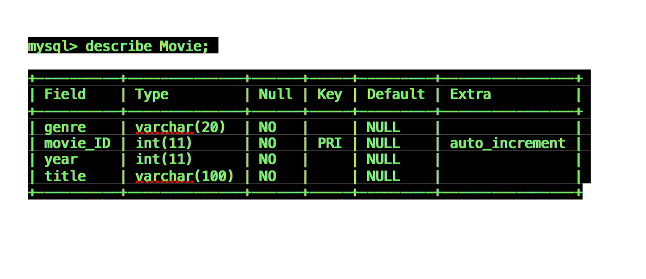
\includegraphics[scale=0.3]{describemovie.png}
		\item{The table attributes that take part in the view: }
		title, genre, year
	\end{itemize}
	\begin{itemize} 
		\item{The table name: }
		Showing
		\item{The table header (all attributes): }
		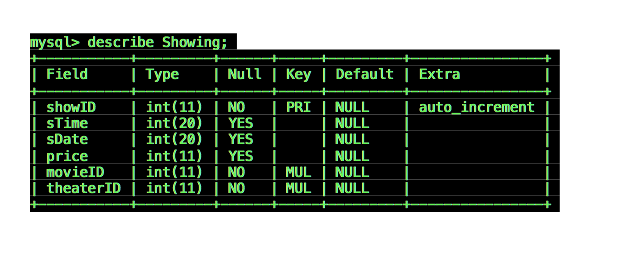
\includegraphics[scale=0.3]{desshowing.png}
		\item{The table attributes that take part in the view: }
		sTime, sDate, price
	\end{itemize}
	\begin{itemize} 
		\item{The table name: }
		Director
		\item{The table header (all attributes): }
		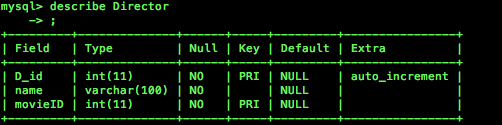
\includegraphics[scale=0.3]{director.png}
		\item{The table attributes that take part in the view: }
		directorname
	\end{itemize}
	\begin{itemize} 
		\item{The table name: }
		Moviegoer
		\item{The table header (all attributes): }
		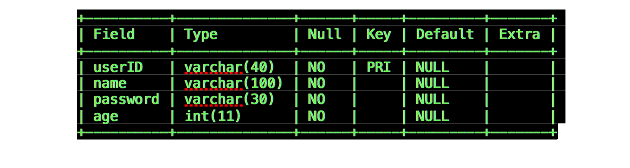
\includegraphics[scale=0.3]{moviegoerdescribe.png}
		\item{The table attributes that take part in the view: }
		username,age
	\end{itemize}
	\begin{itemize} 
		\item{The table name: }
		HasTicket
		\item{The table header (all attributes): }
		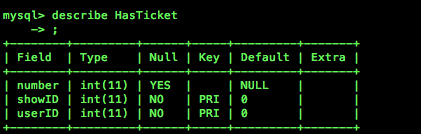
\includegraphics[scale=0.3]{hasticket.png}
		\item{The table attributes that take part in the view: }
		number.
	\end{itemize}
	Please repeat that pattern for every table that takes part in the view.
	\item{The SQL statement used for creating the view: }
	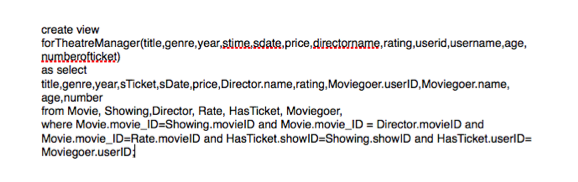
\includegraphics[scale=0.3]{VIEWTHEATER.png}
	\item{The trigger built upon those views (if any): }
	Please insert the triggers as follows.
	\begin{itemize} 
		 \item{The trigger: }
		\includegraphics[scale=0.3]{trigger1.png}
		 \item{The trigger justification (explanation, correlating it to user scenario(s)): }
		 a count variable in which one is added every time a movie is added to the system so any of the managers can know how many movies are added to their movie theater system. a theater manager can check how many movies his theater has 
 	\end{itemize}
\end{itemize}
\end{itemize}
}


\section{Project Highlights.}\label{sec:7. Project Highlights.}
%%%%%%%%%%%%%%%%%%%%%%%%%%%%%%%%%%%%%%%%%%%%%%%%%%%%%%%%%%%%%%%%%%%%%%%%%%%%%%%%%%%%%%%%%%%%%%%%%%%%%%%%%%
\textnormal{
\begin{itemize} 
\item{}
All the related source code should run on the Ilab machines, and should be included with your submission along with the final LaTeX report, as well as the Power Point Presentation.
\item{}
The presentation (7 to 8 minutes) should include the following points (The order of the slides is important):
\begin{enumerate}
\item{}
Title: Project Names (authors and affiliations)
\item{}
Project Goal
\item{}
Outline of the presentation
\item{}
Description
\item{}
A picture is essential. Interface snapshot and users interaction with it
\item{}
Project Stumbling Blocks
\item{}
Data collection, Conceptual Diagram, Integrity constraints
\item{}
Sample of findings
\item{}
Future Extensions
\item{}
Acknowledgements
\item{}
References and Resources used(libraries, languages, web resources)
\item{}
Demo(3 minutes)
 \end{enumerate}
 Please follow the example SuperFinal presentation mock up that is posted on Sakai, for more details.
 \item{}
On July 11th, submission should have taken place. Also you have to be ready to do the presentation (7 to 8 minutes) as well as the demo to show the functionalities of the project (3 minutes): every group member should attend the demo (and presentation) and will have to specify the parts he/she has worked upon, in order to allow us to grade all students with fairness.
\item{}
Thank you, and best of luck!
\end{itemize}
}


\bibliographystyle{IEEEtran}
%\bibliography{IEEEabrv,bib_queyroi_abello2013}
%\bibliography{bib_queyroi_abello2013}

\end{document}


